\subsection{Neonatal \& Perinatal Deaths and Stillbirths}
Neonatal refers to the first 28 days of life after birth. This is a critical period for the baby's development, and neonatal care is essential to ensure their survival and well-being.

Perinatal refers to the period of time surrounding the birth of a baby, typically starting at 22 weeks of gestation and ending seven days after birth. This period includes both the antepartum (before birth) and intrapartum (during birth) periods.

Stillbirth is the term used when a baby is born without signs of life after 20 weeks of gestation. This can happen before, during, or after delivery. Stillbirth is a devastating loss for parents and families and is often a traumatic experience.

In Australia, perinatal deaths are relatively rare, but they remain a significant public health issue.

If we look at the Australia-wide data \textbf{figure \ref{fig:neo-rate}}, \textbf{figure \ref{fig:peri-rate}} \& \textbf{figure \ref{fig:still-rate}} we can see that the neonatal, perinatal, and stillbirth rate are decreasing through the years

\begin{figure}
  \centering
  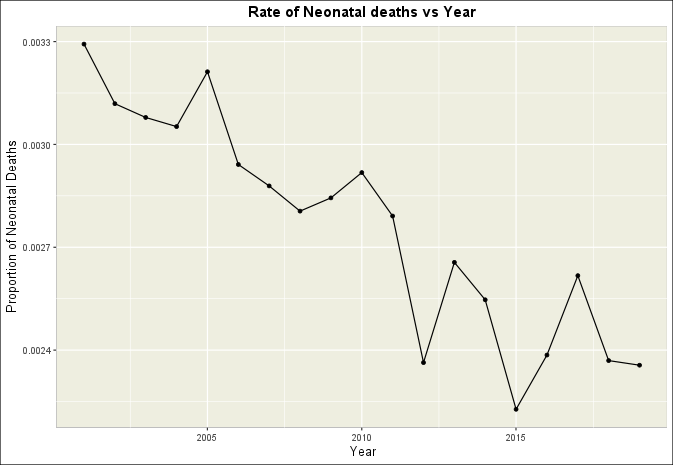
\includegraphics[width=.5\textwidth]{img/aus/kanishka/neonatal_deaths.png}
  \caption{neonatal death rate}
  \label{fig:neo-rate}
\end{figure}

\begin{figure}
  \centering
  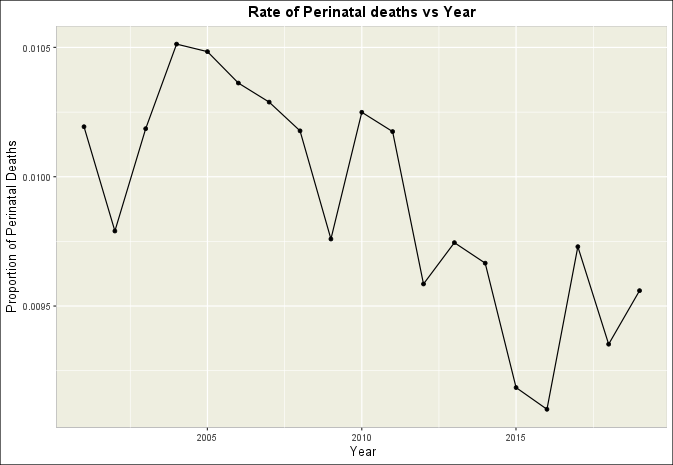
\includegraphics[width=.5\textwidth]{img/aus/kanishka/perinatal_deaths.png}
  \caption{neonatal death rate}
  \label{fig:peri-rate}
\end{figure}

\begin{figure}
  \centering
  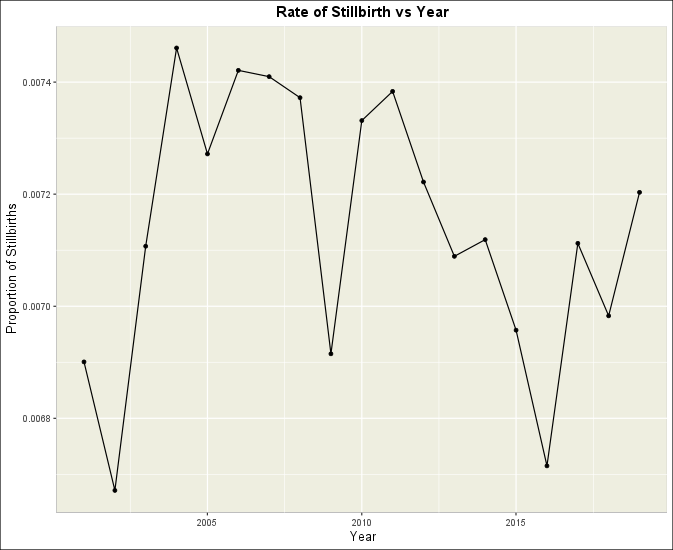
\includegraphics[width=.5\textwidth]{img/aus/kanishka/stillbirth_year.png}
  \caption{stillbirth rate}
  \label{fig:still-rate}
\end{figure}

\subsubsection{Perinatal Deaths vs Mothers' Age}
Perinatal deaths can also happen because of mothers' health factors such as age. To identify how age is contributing to perinatal death we have generated \textbf{Figure \ref{fig:peri_mother}} to try to understand the trend of the data. We can see that perinatal death is significantly high among mothers who are aged below 20. The second biggest group, in this case, is mothers who are aged 40 and over. The group that has consistently low perinatal death is mothers who are aged between 30-34.
\begin{figure}
  \centering
  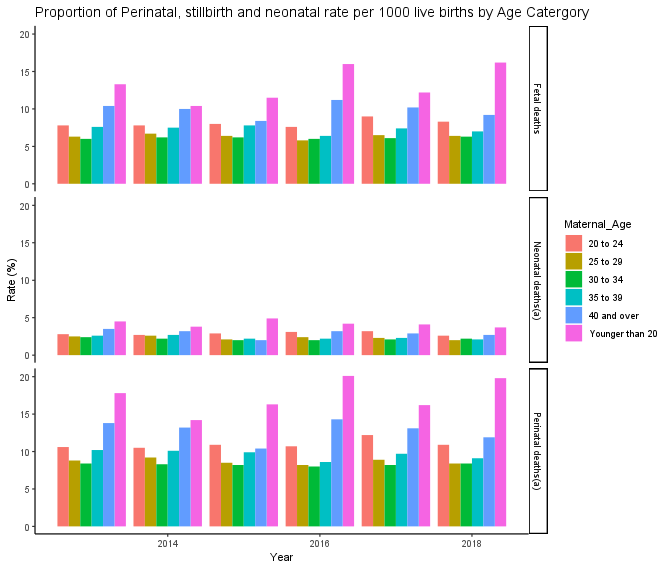
\includegraphics[width=.75\textwidth]{subsections/perinatal_deaths/by_mother_age_baby_death.png}
  \caption{Perinatal death vs Maternal age}
  \label{fig:peri_mother}
\end{figure}
\subsubsection{Child Deaths vs Socio-Economic Area \& Remoteness}
Successful childbirth often depends on parents' socio-economical status \& geographical location since those determine accessibility to better healthcare, medication better antinatal visiting practices.

In \textbf{Figure \ref{fig:peri_state}} we can see that in Queensland and New South Wales, the perinatal death has always been low but in Northern Territory, it has been high through the years. The graph also shows that neonatal deaths are significantly low in every state through the years compared to stillbirths.
\begin{figure}
  \centering
  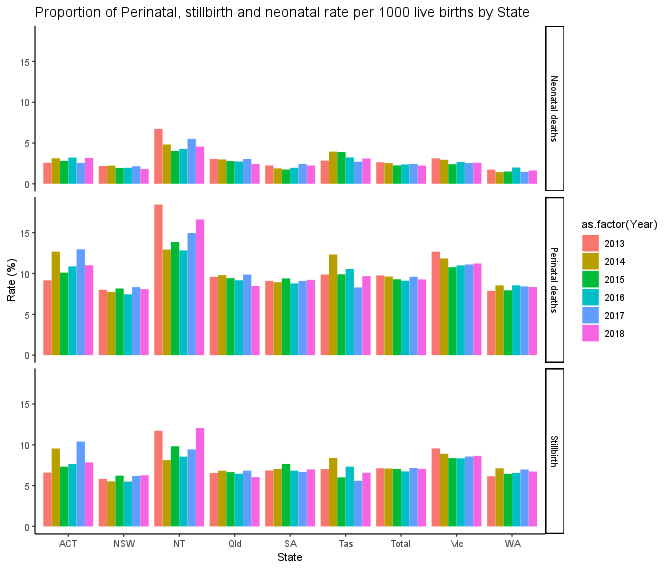
\includegraphics[width=.75\textwidth]{subsections/perinatal_deaths/by_state_birth_baby_death.png}
  \caption{Perinatal death rate per year}
  \label{fig:peri_state}
\end{figure}

To have a deeper understanding, we look into the mother's socio-economic area in \textbf{figure \ref{fig:mother_res}}. Q1 means the most disadvantaged area and Q5 means the least disadvantaged area. It can be clearly observed that the most disadvantaged area has a high mortality rate for all categories of deaths and the least disadvantaged area has the least mortality rate.

\begin{figure}
  \centering
  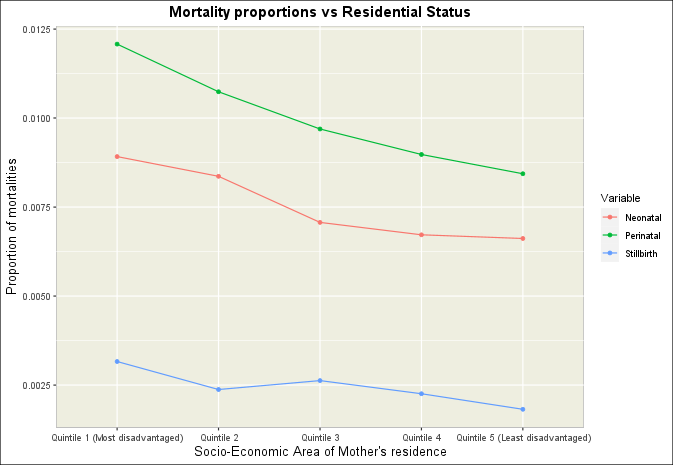
\includegraphics[width=.75\textwidth]{img/aus/kanishka/mortality_residentialStat.png}
  \caption{Socio-economic area of mother's residence}
  \label{fig:mother_res}
\end{figure}

Following that, we wanted to see how the mortality rate was in remote areas in comparison with major cities which are more developed (\textbf{figure \ref{fig:mother_res_remoteness}}). It can be seen that the "Very Remote" areas have the most mortality rate on the other hand major cities have the least death rate.

\begin{figure}
  \centering
  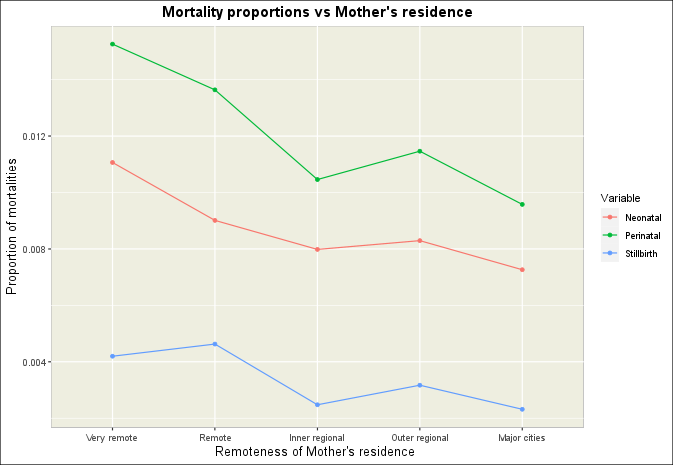
\includegraphics[width=.75\textwidth]{img/aus/kanishka/mortality_mothers_res.png}
  \caption{Remoteness of mother's residence}
  \label{fig:mother_res_remoteness}
\end{figure}